\section{Introduction}

\iflater
\reviewcomment{The paper would be more appealing if strengthened by
  examples. Early on. Specifically, the example application mentioned in the
  last paragraph of Section 4 could be concretized, elaborated, and
  presented first as motivation, then in its actual realisation, up front
  and then as running example along with the formal concepts and
  constructions.}

\reviewcomment{Also concerning applicability, I have a general question
  (also of theoretical interest, I think) about the chosen setup: What about
  more powerful edits? Currently, no recursion or iteration is
  supported. Probably it is not even desirable in full generality, but what
  about iteration at least during navigation? The at(n,e)-edit is only
  one-step navigation. It would not allow to capture something like the
  transitive axes of XPath. Can you capture those, by extending the edit
  language (but maintaining the decidable type-checking)?  }
\fi

Semantic models of bidirectional transformations are generally presented as
transformations between the {\em states} of replicas.  For example, the
familiar framework of asymmetric lenses defines a lens between replicas of
types $A$ and $B$ as a pair of a {\em get} function from $A$ to $B$ and a
{\em put} function from $A \times B$ to $A$.
%
An implementation directly based on this semantics would pass to the {\em
  put} function the entire states of the original $A$ and updated $B$
replicas.

Though pleasingly simple, this treatment falls short of telling a full story
in at least two important ways.
First, it does not explain how the lens should {\em align} the parts of the
old $A$ and the new $B$ so that the parts of $A$ that are ``hidden'' in the
$B$ view retain their positions in the result.  For example, if $A$ and $B$
are both lists of people where each element of $A$ includes a name, address,
and email while the corresponding elements of $B$ give only a name and
address, the user will reasonably expect that inserting a new element at the
head of the $B$ replica will lead to an updated $A$ replica where each
existing name keeps its associated email.  And second, the simple
``classical'' form of asymmetric lenses fails to capture the reasonable
expectation that a small change to the $B$ replica can be transformed into a
change to the $A$ replica using time and space proportional to the size of
the change, not to the sizes of the replicas.  \finishlater{This second point
  sounds a bit bogus, since the system we have in mind is going to have to
  walk over the whole replicas to compute the edit from the original and
  modified structures in the first place. Martin: but then once the edit has been computed one only needs to send a small bit of info}

One way to address at least the first concern is to enrich the basic
structure of a state-based lens with a new input to the {\em put} function,
a data structure that explicitly represents the {\em alignment} between the
original and updated $B$ replicas; this idea forms the basis for {\em
  dictionary lenses}~\cite{Boomerang07}, {\em matching
  lenses}~\cite{Matching10}, and {\em symmetric}~\cite{Diskin-Delta11} and
{\em asymmetric delta lenses}~\cite{diskin2011asymmetric} (based on
\cite{Stevens07}).\finishlater{Need to cite Perdita's relevant papers
  too!}  Another approach is to annotate the $B$ structures themselves with
change information~\cite{HuModels07, Hidaka10}.  However, all these
approaches still involve whole replica states, either as explicit inputs and
outputs of the {\em put} function or implicitly as part of the type to which
a delta belongs.  Thus, it is not clear whether these models can be
implemented in such a way that small changes to a replica are propagated in
time and space proportional to the size of the change.

\finishlater{Maybe we also need
  to cite some of these?  \cite{Meertens98, HuEditor08, MuAlgebraic2004,
    xiong09}}

In earlier work~\cite{HofmannPierceWagner12}, we proposed going a step further and defining
lenses that work exclusively with edits.  We defined a semantic model called
{\em edit lenses} in which the sets of source and target replicas $A$ and
$B$ are enriched with monoids of {\em edits} and a lens's {\em get} and {\em
  put} functions map edits to edits.  This work was carried out in an
abstract algebraic setting where the actual data structures being
transformed and the exact shapes of edits to them were left unspecified; in
this setting, we showed how a number of familiar constructions on
lenses---products, sums, etc.---could be carried out.

The present paper takes a first step
toward instantiating this abstract semantic
model with concrete data structures and a concrete notion of edits.  The
data model we choose is a very common and expressive one: unordered,
edge-labeled trees---called {\em information trees} by Dal Zilio {\em et
  al}~\cite{DalzilioS:POPL04}. These can encode a variety of data formats,
including XML-style trees, their original application.
Such trees can also be used to represent graphs
\cite{UnQL96,Hidaka10} by unrolling up to bisimulation. This paper thus
makes a first step towards general edit languages for trees.  Our edit
operations include, in particular, insertion and deletion of subtrees and
renaming of edges; we show how these give rise to edit languages on tree
languages and can thus be used to instantiate the framework of {edit
  lenses} so as to yield bidirectional synchronization between information
trees.

Our main technical result is that weakest preconditions of our edits
can be effectively computed for sets of information trees specified by
sheaves automata. This allows for effective ``type checking'' of edits
and thus permits automatic checks that an edit language for trees
presented as sequences of atomic edits does indeed preserve acceptance by a
given sheaves automaton.

The present work is thus a first step; we hope that the introduction
of tree automata into the world of editing and synchronization will
also lead to high-level support for constructing edit lenses
themselves and for checking their soundness, but this remains future
work.

\section{Examples}
\label{sec:examples}
% TODO: could use the actual edit language for sums from our delta paper as
% a motivating contrasting example! Plus we get to point out that there is
% no One Translation -- can check that many translations all work out, and
% the high-level lenses get to operate on the high-level operations

As a running example, we will use a simplified model of a filesystem. In our
filesystem, there are three kinds of objects: directories, files, and
bit strings. In our simple model, we will identify files by a name that
starts with a lower case letter; files will contain bit strings. For
example, here's a simple file named ``greeting'':
\[\Open\Label{greeting}\To\Label{0110100001101001}\Close.\]
We will identify directories by a name that starts with an upper case letter;
directories contain filesystems. A filesystem is a collection of files and
directories. For example, here is a simple filesystem:\bcp{To me, commas
  look better at the ends of lines (in a proportional-width font)}
\[
\begin{array}{c@{}r@{\;}l@{\;}l}
    \Open&\Label{Etc} &\To&\Open\Label{passwd}\To\Label{0110} \\
         &            &   &\;,  \Label{alternatives}\To\Label{010}\Close \\
    ,    &\Label{foo} &\To&\Label{1010110}\Close \\
    \Close
\end{array}
\]
Call this example filesystem $E$.

In addition to modeling the current state of a file system, we will want to
model file system operations like creating, deleting, and moving files and
directories. To do so, we will define a collection of edits and an operation
that applies edits to filesystems. To create new files and directories at
the top level, we define the $\Insert$ operation, which takes a filesystem
to merge into the existing one. For example, to create a ``/home/john'' directory (with no files
or directories inside) in our example filesystem, we would use:
\[\Insert(\Open\Label{Home}\To\Open\Label{John}\To\Open\Close\Close\Close)\cdot E=
\begin{array}[t]{c@{}r@{\;}l@{\;}l}
    \Open&\Label{Etc} &\To&\Open\Label{passwd}\To\Label{0110} \\
         &            &   &\;,  \Label{alternatives}\To\Label{010}\Close \\
    ,    &\Label{Home}&\To&\Open\Label{John}\To\Open\Close\Close \\
    ,    &\Label{foo} &\To&\Label{1010110}\Close \\
    \Close
\end{array}
\]
For simplicity, we will say that any name clashes result in failure; for
example, trying to apply the edit $\Insert(\Open\Label{Etc}\To\Open\Close\Close)$ to $E$
would be undefined.

To allow the creation of files in other places than at the root, we will
define another edit operation, $\At(n,e)$, which applies edit $e$ to the
subpart of the filesystem rooted at $n$. For example, to add the
``/etc/dbus'' file to our example filesystem, we would
\[\At(\Label{Etc},\Insert(\Open\Label{dbus}\To\Label{10101}\Close))\cdot
E\]
which would result in
\[
\begin{array}{c@{}r@{\;}l@{\;}l}
    \Open&\Label{Etc} &\To&\Open\Label{passwd}\To\Label{0110} \\
         &            &   &\;,  \Label{alternatives}\To\Label{010} \\
         &            &   &\;,  \Label{dbus}\To\Label{10101}\Close \\
    ,    &\Label{Home}&\To&\Open\Label{John}\To\Open\Close\Close\Close \\
    ,    &\Label{foo} &\To&\Label{1010110}\Close \\
    \Close.\!\!
\end{array}
\]

To support moving files and directories around the filesystem, we
define two more kinds of edits, $\Hoist$ and $\Plunge$, which float and sink
entire subtrees one level. For example, if we wanted to move the file
``/foo'' into ``/home/john'', we might first move it into ``/home'' with
$\Plunge(\Label{Home},\Label{foo})$, then move it into ``/home/john'' with
$\At(\Label{Home},\Plunge(\Label{John},\Label{foo}))$.

To round out our operations, we also define $\Delete$ and $\Rename$
operations, whose behaviors are predictable from their names.
%
Besides renaming files and directories in-place, $\Rename$ has a more
subtle use. Consider the following filesystem:
\[
\begin{array}{c@{}r@{\;}l@{\;}l}
    \Open&\Label{Bin}&\To&\Open\Label{cat}\To\Label{0000}\Close\\
    ,    &\Label{Usr}&\To&\Open\Close\\
    ,    &\Label{Opt}&\To&\Open\Label{Bin}\To\Open\Label{coq}\To\Label{1111}\Close\Close\Close
\end{array}
\]
Call this filesystem $E'$. Now, we decide we would like to move the
``/opt/bin'' directory into ``/usr''. Naively, we would like to hoist
``/opt/bin'' to ``/bin'', then plunge ``/bin'' to ``/usr/bin''; however, the
first hoist operation would result in a name clash with the existing
``/bin''. One way we can avoid this is to temporarily rename $\Label{Bin}$
to a secret name which definitely will not clash:
\begin{align*}
\At(\Label{Usr},\Rename(\Label{\#Bin},\Label{Bin}))\cdot& \\
\Plunge(\Label{Usr},\Label{\#Bin})\cdot\Hoist(\Label{Opt},\Label{\#Bin})\cdot& \\
\At(\Label{Opt},\Rename(\Label{Bin},\Label{\#Bin}))\cdot& E'
\end{align*}
This sequence of edits is now quite robust: it will work in any filesystem
that has both ``/opt/bin'' and ``/usr'' but no ``/usr/bin''. On the other
hand, notice that this sequence of edits temporarily breaks some of the
invariants of filesystems: for a time, there are subtrees that are not bit
strings, directories, or files.
%
For a more
 interesting examples where invariants need to be temporarily broken consider that in the spirit of B-trees we impose maximum and minimum numbers of files to be held by any one non-root directory. Then, in order to insert a file, it may be necessary to split a directory into two using a long sequence of basic edits only at the end of which the invariant will be restored.

During our exploration of filesystems and how to represent edits, we have
briefly seen several ways that edits can ``go wrong''. There are three
failure classes of interest:
\begin{enumerate}
    \item It may be clear that a particular edit can never apply to a valid
        filesystem; e.g. the edit $\Delete(\Label{\#foo})$ that tries to
        delete a file with an invalid name.
    \item An edit may be applicable to some filesystems but break filesystem
        invariants and never properly restore them. We would like to prevent
        this without ruling out edits which \emph{do} properly restore
        invariants.
    \item There may be edits that apply to some filesystems correctly but
        fail on others; e.g. the edit
        $\Insert(\Open\Label{Foo}\To\Open\Close\Close)$ that inserts a
        new directory works on any filesystem that does not yet have a
        ``/foo'' directory.
\end{enumerate}
In this paper, we discuss a way to detect the first two classes of failures.

\section{Trees and sheaves automata}

This section introduces some notations and definitions that we need in the
sequel.  Some of the descriptions are taken
from~\cite{Foster:FTL}.\finishlater{Can we rewrite so that we don't need to
  confess to plagiarizing them? :-)}

\subsection{Trees}
We assume a finite alphabet $\Sigma$ and consider unordered trees whose
edges are labeled by $\Sigma^*$. We write trees with a pair of
braces $\Open\Close$ for each node; each subtree is written
$\Label{n}\To t$, where $\Label{n}$ names the edge that leads to the subtree
$t$. To reduce clutter, we abbreviate the tree
$\Open\Label{n}\To\Empty\Close$ to just $\Label{n}$ when no confusion
arises. For example, here is an explicit tree with two children labeled
``home'' and ``etc''\dots
\[\Open\Label{Home}\To\Open\Label{John}\To\Empty\Close,\Label{Etc}\To\Open\Label{passwd}\To\Empty\Close\Close\]
\dots{}and its abbreviated form:
\[\Open\Label{Home}\To\Label{John},\Label{Etc}\To\Label{passwd}\Close\]
We write $t(n)\Defined$ to indicate that tree $t$ has child $n$,
$t(n)\Undefined$ to indicate that tree $t$ does not have child $n$, and
$t(n)$ for the child under the edge labeled $n$. We write $\Domain(t)=\{n \mid
n \in \Sigma^* \land t(n)\Defined\}$. The expression $t[n \To t']$ describes the
tree that agrees with $t$ everywhere, except that its child under label $n$
is $t'$.  The expression $t \Except \{n_1,n_2,\ldots,n_k\}$ describes the
tree that is
undefined at $n_1,n_2,\ldots,n_k$ but agrees with $t$ everywhere else. When
context makes it clear that $n$ is a name, we write $t \Except
n$ to mean $t \Except \{n\}$. To simplify the definition of partial
functions, we take an expression like
$t[n \To E]$ when $E$ is undefined to be undefined itself.

\finish{we need plunge!!!}
\subsection{Tree edits}
The set of {\em atomic tree edits} is defined as
follows\footnote{The edits presented here are fairly simple. One might
  wonder whether more complicated edits---for example, ones that allowed
  recursion or tree queries---could also be supported in this framework. For
  the moment, we take the stance that these more complicated edits might be
  provided by some external editing tool, but that they should then be
  ``compiled down'' to sequences of atomic edits.  This is a point that
  deserves further consideration.} (where $e$ ranges over edits, $t$ over
trees, and $m$ and $n$ over names):
\[
e \;\;::= \;\;
\Insert(t)  \;\;|\;\;
\Hoist(m,n) \;\;|\;\;
\Delete(m) \;\;|\;\;
\Rename(m,n) \;\;|\;\;
\At(n,e)
\]
\finishlater{Might consider $\Delete(r)$ for $r$ a language.}
\finishnow{And {\em plunge}!}
%
The application of an atomic edit $e$ to a tree $t$ is either undefined
($\bot$) or a new tree defined as follows:
\begin{align*}
    \Insert(t') \cdot t &=
        t \cup t' &&
        \mbox{if }\Domain(t)\cap\Domain(t')=\emptyset \\
    \Hoist(m,n) \cdot t &=
        t[m \To t(m) \Except n,n \To t(m)(n)] &&
        \mbox{if }t(m)(n)\Defined \land\; t(n)\Undefined \\
    \Delete(n) \cdot t &=
        t \Except n &&
        \mbox{if }t(n) = \Empty\footnotemark\\
    \Rename(n,n') \cdot t &=
        (t \Except n)[n' \To t(n)] &&
        \mbox{if }t(n)\Defined \land\; t(n')\Undefined \\
    \At(n,e) \cdot t &=
        t[n \To e \cdot t(n)] &&
        \mbox{if }t(n)\Defined \\
    e \cdot t &= \bot && \mbox{in all other cases}
\end{align*}
\footnotetext{Our $\Delete$ operation deletes a single, explicitly named
leaf node, but this is not a fundamental restriction. Operators that delete
entire subtrees or all children in a regular language seem like reasonable
alternate design choices.}

Tree edits are sequences of atomic edits. We overload $\cdot$ as tree
edit application, which is the natural lifting of atomic edit application to
sequences:
\begin{align*}
    \left<\right> \cdot t &= t \\
    \left<a_1,\ldots,a_n\right> \cdot t &=
        \left<a_1,\ldots,a_{n-1}\right>\cdot(a_n \cdot t)
\end{align*}

\subsection{Sheaves formulae and automata}

Conceptually, a {\em sheaves automaton} consists of a set of states, each
associated with a {\em sheaves formula}; each sheaves formula describes a
set of trees by specifying which names may occur as immediate child edges
and, for each one, an automaton state that describes the subtree found
beneath it.

To describe sheaves automata more formally, we must first fix a formalism
for writing down arithmetic constraints. We use Presburger arithmetic---the
decidable first-order theory of the naturals with addition but without
multiplication---for this purpose.\footnote{Here we follow the lead of
\cite{Foster:FTL} and \cite{DalzilioS:POPL04}. Presburger arithmetic is
quite an expressive logic, and it is possible that a simpler fragment
suffices, but we leave an investigation of this possibility to future
work.} Expressions in Presburger arithmetic include
constants, variables, and sums, and formulae include equalities
between expressions, boolean combinations of formulae, and quantified
formulae:
\begin{align*}
    m &::= 0 \mid 1 \mid 2 \mid \cdots \\
    v &::= m \mid x_m \mid v+v \\
    \phi &::= v = v \mid \phi \lor \phi \mid \phi \land \phi
    \mid \lnot \phi \mid \exists \phi
\end{align*}
\noindent
We use a de Bruijn representation---a variable \(x_j\) within the
scope of \(k\) quantifiers represents the \((j-k)\)th free variable if
\(j \geq k\), and otherwise is bound by the \(j\)th enclosing
quantifier, counting from the inside-out.

The semantics of a Presburger formula is the set of vectors of
naturals that satisfy it. \finishlater{The appendix of the FTL paper gives
  this defn in detail, if needed.}
%
We write $\bar c \vDash \phi$ for formula satisfaction, substituting
$c_i$ for $x_i$, and $\Free(\phi)$ for the set of free variables in $\phi$.

\newcommand{\ELEMENT}[2]{(#1, #2)}
\newcommand{\FORMULA}[3]{(#1, #2, #3)}
\newcommand{\VECTOR}[1]{(#1)}
\newcommand{\PNEG}[1]{\lnot{#1}}
\newcommand{\E}{E}

Next, a {\em sheaves automaton} comprises a finite set of states together
with a mapping \(\Gamma\)
from states to \emph{sheaves formulae}. The transition behavior from a
state is given by the sheaves formula{} associated with it in
\(\Gamma\). Each sheaves formula has three components---a Presburger formula
$\phi$, a list of regular languages $\bar r$, and a list of successor states
$\bar s$. The pair of a regular language $r_i$ and the successor state $s_i$
at the corresponding index is called an \emph{element}. The operation of a
sheaves automaton is like a bottom-up regular tree automaton. Let \(t\) be a
tree and \(s\) be an automaton state with \(\Gamma(s) =
\FORMULA{\phi}{\left<r_0,\ldots,r_k\right>}{\left<s_0,\ldots,s_k\right>}\). For
each \(i\) in the range \(0\) to \(k\), let \(c_i\) be the number of
children \(n \in \Domain(t)\) for which \(n \in r_i\) and \(t(n)\) is
accepted by \(s_i\). Then \(t\) is accepted by \(s\) iff
\(\VECTOR{c_0,\dots,c_k} \models \phi\).

Note that the integers that represent variables in de Bruijn notation
give the correspondence between free variables in \(\phi\) and
elements---the constraint on \(x_i\) controls the number of children
whose name matches \(r_i\) with subtrees accepted by \(s_i\).

In the following, it will sometimes be convenient to treat elements (and the
corresponding Presburger variables in the sheaves formula) as if they were
indexed by some set with more structure than the natural numbers.  This is
perfectly reasonable, provided there is an injective mapping from the
structured set to the naturals. When it is clear that such an injective
mapping $f$ exists (and in particular especially when the structured set is
finite) we will leave the mapping unspecified and simply use values from the
structured set as subscripts to the collections $\bar r$ and $\bar s$ as
well as any Presburger variables, understanding $r_{v}$ to stand for
$r_{f(v)}$.
\dmwit{Does this convention need to be explained more? Also, how hard can we
abuse this? (Are there more places where notation can be cleaned up with
this trick?)}

Sheaves automata and sheaves formulae{} are subject to some well-formedness
conditions. A sheaves formula{} \(\FORMULA{\phi}{\bar r}{\bar s}\) with
\(|\bar r| = k\) is well-formed iff $|\bar s| = k$; the free variables of
\(\phi\) are
%
\(\{x_0,\dots,x_{k-1}\}\); the elements are pairwise disjoint---i.e.,
if there exists a tree accepted by both \(s_i\) and \(s_j\), then the
regular languages denoted by \(r_i\) and \(r_j\) are disjoint; and the
elements are generating---i.e., for every tree \(t\) and label \(n \in \Domain(t)\)
there is an \(i\) such that \(n \in r_i\) and
\(t(n)\) is accepted by \(s_i\). A list of elements obeying these
conditions is called a \emph{basis}. A sheaves automaton{} is well-formed iff
every sheaves formula{} in the range of \(\Gamma\) is well-formed.
%
These well-formedness conditions guarantee two properties.  First,
because the elements are non-overlapping, every tree has a unique
decomposition over the basis, which means that the semantics of a
sheaves automaton is well-defined. Second, because the elements generate the set
of all tree slices, certain constructions are simple. For example,
\(\FORMULA{\phi}{\bar r}{\bar s}\) and \(\FORMULA{\PNEG{\phi}}{\bar
r}{\bar s}\) accept complementary sets of trees.

\newcommand{\PEQUAL}[2]{#1\!=\!#2}
\newcommand{\TRUTH}{\top}
\newcommand{\TRUE}{\TRUTH}
\newcommand{\name}{\Label}
\newcommand{\RNEG}[1]{\overline{#1}}

One of the simplest automata is the one that accepts any tree. It has a
single state, which we will name $\TRUE$, and whose transition relation is
given by $\Gamma(\TRUE)=\FORMULA{\PEQUAL00}{[\Sigma^*]}{[\TRUE]}$. In fact,
having such a state is so convenient that we will assume in the remainder of
the paper that every automaton has a state named $\TRUE$ that accepts all
trees (and consequently omit the definition of $\Gamma(\TRUE)$). As a more
exciting example, the set of trees
\[
\{
\Open\Close ,\; \Open\Label{a},\Label{b}\Close
\}
\]
is described by the automaton{} state \(s\), where \(\Gamma(s)\) is:
\[
\left(
\begin{array}{l}
((\PEQUAL{x_0}{0} \wedge \PEQUAL{x_1}{0}) \vee (\PEQUAL{x_0}{1} \wedge \PEQUAL{x_1}{1})) \wedge (\PEQUAL{x_2}{0}),\\
% don't want this next [ to be interpreted as beginning an optional argument
% to the preceding \\
{}[\name{a},\name{b},\RNEG{\{\name{a}, \name{b}\}}],\\
{}[\TRUE,\TRUE,\TRUE]
\end{array}
\right)
\]
To see this, observe that the constraints on \(x_0\) and
\(x_1\) force the number of children described by the elements
\(\ELEMENT{\name{a}}{\TRUE}\) and \(\ELEMENT{\name{b}}{\TRUE}\) to
both be \(0\) or both be \(1\), and that the constraint on \(x_2\) forces the
number of children belonging to the final element to be \(0\), that is,
there are no edge labels other than \(\name{a}\) or \(\name{b}\).

% Now
% \emph{Elements}, \emph{sheaves formulae}, and \emph{sheaves automata} are
% defined mutually recursively.
% \mh{Are Elements ever used?}
% \begin{description}
%     \item[element] a pair $r[s]$ of a regular language $r$ over $\Sigma$ and
%         a state $s$ of an automaton
%     \item[sheaves formula] a triple $(\phi,\bar r,\bar s)$ of a Presburger
%         formula $\phi$, a sequence of regular languages $r_i$ over $\Sigma$,
%         and a sequence of automaton states $s_i$, such that
%         $\Free(\phi)=|\bar r|=|\bar s|$
% \mh{$\Free(\phi)$ is a set and $|\bar r|$ is a number.}
%     \item[sheaves automaton] a triple $(S,s_0,\Gamma)$ of a set of states
%         $S$, an initial state $s_0\in S$ and a mapping $\Gamma$ from $S$ to
%         sheaves formulae subject to a well-formedness condition (discussed
%         below)
% \end{description}
% The relation $A,s \vdash t$ tells when automaton $A$ accepts tree $t$
% starting at state $s$. When
% \begin{align*}
%     A &= (S,\Gamma) \\
%     s &\in S \\
%     \Gamma(s) &= (\phi,\bar r,\bar s) \\
%     c_i &= \mbox{the number of labels $n \in r_i\cap\Domain(t)$ for which
%     $A,s_i \vdash t(n)$}
% \end{align*}
% then $A,s \vdash t$ iff $\bar c \vDash \phi$. A sheaves formula $(\phi,\bar
% r,\bar s)$ is well-formed in automaton $A$ when it specifies a partition of the set
% of all trees, that is, when:
% \begin{itemize}
%     \item For all trees $t$ and labels $n$, there is some $i$ for which
%         $n \in r_i$ and $A,s_i \vdash t$.
%     \item If there is a tree $t$ and indices $i \ne j$ such that $A,s_i
%         \vdash t$ and $A,s_j \vdash t$, then $r_i \cap r_j = \emptyset$.
% \end{itemize}

The relation $A,s \vdash t$ tells when automaton $A$ accepts tree $t$
when started at state $s$.
We often write sheaves automata as $A = (S,s_0,\Gamma)$, where $s_0$ is a
distinguished initial state.
We then write $A\Vdash t$ to mean $A,s_0\vdash t$.
%
We also write $L(A)=\{t\mid A\Vdash t\}$ for the language accepted by
automaton $A$.

\section{Weakest preconditions of edits}
So far, we have reviewed a definition for trees and a notion of
type-checking for trees, namely, sheaves automata. We have also given a
definition for tree edits; what remains is to give a notion of type-checking
for tree edits. The type of a tree edit will have two tree types, one
describing source trees and one describing target trees. Below, we will show
how to take a target tree type $T$ and an atomic edit $e$ and infer a type $S$
for which applying $e$ to an $S$ tree produces a $T$ tree; we will argue
that this $S$ is maximal and therefore checking that $e$ has a given type
$S' \to T$ amounts to checking that $S'$ is a subtype of $S$.

Let $A,B$ be sheaves automata and $e$ be a tree edit. We write $e:A\rightarrow
B$ to mean that whenever $A\Vdash t$ and $e\cdot t$ is defined we have $B\Vdash e\cdot t$.

We now define for each atomic edit $e$ and automaton $A$ a new automaton
$e\cdot A$ such that $t\in L(e\cdot A)$ iff $e\cdot t\in L(A)$ whenever
$e\cdot t$ is defined, that is, $e \cdot A$ is an automaton representing the
weakest precondition that ensures that applying edit $e$ will result in a
tree of type $A$. Formally: $L(e\cdot A)=\{t\mid e.t\Defined \Rightarrow
e.t\in L(A)\}$.  It is then clear that $e:A\rightarrow B$ iff $L(A)\subseteq
L(e\cdot B)$ (notice that if $e.t$ is undefined then, trivially, $t\in
L(e.A)$). Language inclusion of sheaves automata being
decidable~\cite{DalzilioS:POPL04}, this then implies a decision procedure
for $e:A\rightarrow B$ and in particular for deciding whether a given tree edit
belongs to $A \to A$.

\begin{theorem}
Let $A=(S,s_0,\Gamma)$ be a sheaves automaton and $e$ be an atomic
edit. There exists a sheaves automaton $e\cdot A = (S',s_0',\Gamma')$ such
that $t\in L(e\cdot A)$ iff $e\cdot t$ is undefined or $e\cdot t\in L(A)$.
Moreover, $e\cdot A$ can be effectively obtained from $e$ and $A$.
\end{theorem}

\begin{proof}
\finish{expand this proof sketch with some more explanation}
The construction proceeds in two stages. First, we define for each edit $e$ a sheaves automaton $D_e$ such that $L(D_e)=\{t\mid e\cdot t\Undefined\}$.

Then, for each edit $e$, we construct a sheaves automaton $e\star A$
such that for all $t$ with $e\cdot t\Defined$ one has $e\star A\Vdash
t\iff A\Vdash e\cdot t$. We then define the desired automaton $e\cdot
A$ so that $L(e\cdot A)=L(D_e)\cup L(e\star A)$ using the union
construction from \cite{DalzilioS:POPL04}.

Given this strategy, the remaining definitions are essentially a programming
exercise.\finish{Reviewer suggests picking one of the atomic operations --
  e.g. Insert -- and describing the following programming exercise pictorially.}
\begin{itemize}
\item $e=\Insert(t')$. For $D_e$ we need to check that some top-level label
from $t'$ is present. If the top-level labels are, say, $r_0\dots r_n$ and $r_{n+1}$ is
$\Sigma^*\setminus \{r_0,\dots,r_n\}$ then the sheaves formula
$(0\ne\sum_{i=0}^n x_i,\bar r,\bar\top)$
achieves the purpose when attached to the initial state of $D_e$.

To build $e\star A$ we add a fresh state $s_0'$ that is just like $s_0$
except that it has already ``seen'' the subtree $t'$. That is, if
$\Gamma(s_0) = (\phi,\bar r,\bar s)$ and $c_i$ is the number of labels $n
\in r_i \cap \Domain(t')$ for which $A,s_i \vdash t'(n)$, then we define
\begin{align*}
    S' &= S \cup \{s_0'\} \\
    \phi' &= \phi[x_i + c_i/x_i] \\
    \Gamma' &= \Gamma[s_0' \To (\phi',\bar r,\bar s)]
\end{align*}
where $\phi[e/x]$ is the formula $\phi$ with expression $e$ substituted for
variable $x$.
% \mh{Must also take care of the case $e\cdot t$ undefined. Namely, in this case we want to accept straightaway!}
% \dmwit{I think the way we set up the definitions this issue doesn't come up:
% we only compare the ``truthiness'' of $t \in L(e \cdot A)$ and $e \cdot t
% \in L(A)$ when $e \cdot t$ is defined.
% }
% \mh{Well, we want to know whether
% $\forall t.e.t\Defined \wedge t\in L(A) \Rightarrow e\cdot t\in L(B)$. To this end, we define $e\cdot A$ in such a way that the latter statement is logically equivalent to $L(A)\subseteq L(e\cdot B)$, i.e., $\forall t.t\in L(A)\Rightarrow t\in L(e\cdot B)$.  This then requires that a $t$ with $e\cdot t$ undefined is always contained in $L(e\cdot B)$ for otherwise, we might get spurious artifacts in the case where such a $t$ happens to be in $L(A)$. To wit, suppose that $e$ is the everywhere undefined edit. Clearly, $e:A\rightarrow B$ holds for all $A$ and $B$, so $e\cdot B$ must contain all trees rather than being the empty set.

% I guess we want to say that for given edit $e$ we can always design a sheaves automaton $A_e$ such that $A_e\vdash t\iff e\cdot t\Undefined$. We can then form the union of what we have and this guy.
% }

\item $e=\Hoist(m,n)$. Suppose $\Gamma(s_0)=(\phi,\bar r,\bar s)$.
\finish{talk a bit about this figure to give some intuition about what we
should do}
\begin{figure}
    \begin{center}
        \begin{subfigure}[b]{0.4\textwidth}
            \begin{center}
                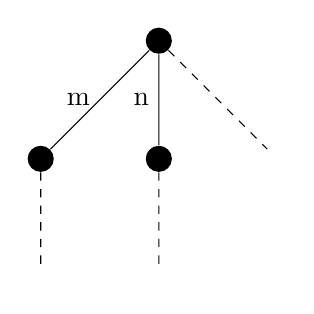
\begin{tikzpicture}
                    \node[circle,fill] {}
                        child {
                            node[circle,fill] {}
                                child[dashed] { node {} }
                            edge from parent node[left] {m}
                        }
                        child {
                            node[circle,fill] {}
                                child[dashed] { node {} }
                            edge from parent node[left] {n}
                        }
                        child[dashed] { node {} }
                        ;
                \end{tikzpicture}
            \end{center}
            \caption{The trees automaton $A$ accepts.}
            \label{fig:hoist-input}
        \end{subfigure}
        \begin{subfigure}[b]{0.4\textwidth}
            \begin{center}
                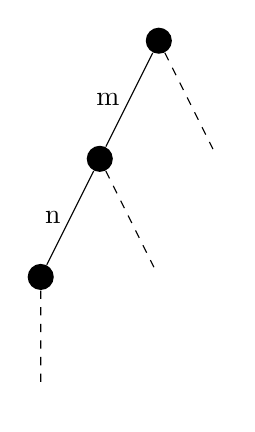
\begin{tikzpicture}
                    \node[circle,fill] {}
                        child {
                            node[circle,fill] {}
                                child {
                                    node[circle,fill] {}
                                        child[dashed] { node {} }
                                    edge from parent node[left] {n}
                                }
                                child[dashed] { node {} }
                            edge from parent node[left]{m}
                        }
                        child[dashed] { node {} }
                        ;
                \end{tikzpicture}
            \end{center}
            \caption{The trees $\Hoist(m,n)\cdot A$ should accept.}
            \label{fig:hoist-output}
        \end{subfigure}
    \end{center}
    \caption{the $\Hoist$ operation}
    \label{fig:hoist}
\end{figure}
The high-level plan for $e\star A$ is to add some new states for each state that the
$m$-branch could be accepted under that tell which state the $n$-branch was
accepted under. To this end, define sets $I_m$ and $I_n$ so that $m \in r_i$
iff $i \in I_m$ and likewise $n \in r_i$ iff $i \in I_n$. We now perform the
following modifications:

\finish{hm, this is a bit informal -- seems we should turn this into symbols
a bit}
\begin{itemize}
    \item Add a fresh state $s_0'$, making it the initial state, and letting it
        initially be a copy of $s_0$.
    \item Remove the $I_m$ languages (and their associated successor states)
        from the sheaves formula associated with $s_0'$.
    \item For each $(i,j) \in I_m \times I_n$, add a new regular language which is a
        copy of the original $r_i$ and whose successor state is a copy of
        the automaton that accepts the language of trees that can be split
        into an $n$ part accepted by $s_j$ and a remainder accepted by
        $s_i$. Name the indices of the regular languages and successor states added by
        this operation $k_{ij}$.
    \item Modify the Presburger formula associated with $s_0'$ to reflect
        the changes above: for each $i \in I_m$, replace occurrences of
        $x_i$ with $\sum_j x_{k_{ij}}$, and for each $j \in I_n$, replace
        occurrences of $x_j$ with $\sum_i x_{k_{ij}}$. (If $i \in
        I_m \cap I_n$ for some $i$, then these two operations coincide,
        because of the partitioning property of sheaves formulae.)
\end{itemize}

For $D_e$, we must check that the tree $t$ has $t(m)(n)\Undefined$ or
$t(n)\Defined$; this is easily done by defining $D_e=(\{\top,s,n,\bar n\},s,\Gamma)$
where
\begin{align*}
    \Gamma(s) &= (x_0=0\lor x_1\ne0\lor x_2\ne0,
        [\{m\}[n],\{m\}[\bar n],\{n\}[\top],\overline{\{m,n\}}[\top]]) \\
    \Gamma(n) &= (x_0\ne0,[\{n\}[\top],\overline{\{n\}}[\top]]) \\
    \Gamma(\bar n) &= (x_0=0,[\{n\}[\top],\overline{\{n\}}[\top]]).
\end{align*}

\item $e=\Delete(n)$. The automaton that accepts exactly the tree $\Open n
\To \Empty \Close$ is easy to construct; call this automaton $A'$. We then
define $D_e = \lnot(\top+A')$ using the constructions described
in~\cite{Foster:FTL}. For $e\star A$,
 remove $n$ from each of the $r_i$. Then add an extra condition guarded by
 $n$. Place no constraint on the corresponding cardinality. Leave the other
 cardinalities as they were.


\item $e=\Rename(n,n')$. Suppose $\Gamma(s_0)=(\phi,\bar r,\bar s)$. Choose
a fresh $s_0'$ and define
\begin{align*}
    r'_i &= \cond{
        r'_i \cup \{n\} & n' \in r'_i \\
        r'_i \setminus \{n\} & n' \notin r'_i
        } \\
    S' &= S \cup \{s_0\} \\
    \Gamma' &= \Gamma[s_0' \To (\phi,\overline{r'},\bar s)]
\end{align*}
Then this new automata counts any $n$-rooted subtree as if it were an
$n'$-rooted one instead.

We should briefly argue that the sheaves formula given for $s_0'$ is
generating and pairwise disjoint.  It is generating: take any tree $t$ and
name $n'' \in \Domain(t)$, and apply the definition of ``generating'' to the
original sheaves formula using the tree $[n' \To t(n'')]$ if $n'' = n$ or
using the tree $[n'' \To t(n'')]$ if not. It is pairwise disjoint: consider
$r'_i[s_i]$ and $r'_j[s_j]$ for which both $s_i$ and $s_j$ accept tree $t$.
Take any name $n'' = n$ (resp. $n'' \ne n$).  Since the original sheaves
formula is pairwise disjoint, at most one of $r_i$ and $r_j$ contain $n'$
(resp. $n''$), hence at most one of $r'_i$ and $r'_j$ contain $n''$.

% It is generating: take any tree $t$ and name $n'' \in \Domain(t)$. Either
% $n'' = n$ or not. If $n'' = n$, there is some $i$ for which $n' \in r_i$ and
% $t(n'') \in s_i$ (by applying the fact that the original sheaves formula is
% generating to the tree $[n' \To t(n'')]$), hence $n'' \in r'_i=r_i \cup
% \{n''\}$ and $t(n'') \in s_i$.  Otherwise, $n'' \ne n$ and again applying
% the fact that the original formula is generating, this time to the tree
% $[n'' \To t(n'')]$, tells us that there some $i$ for which $n'' \in r_i$ and
% $t(n'') \in s_i$. Since $n'' \ne n$, we know $n'' \in r_i$ iff $n'' \in
% r_i'$, as desired.
%
% It is pairwise disjoint: consider $r'_i[s_i]$ and $r'_j[s_j]$ for which
% both $s_i$ and $s_j$ accept tree $t$. Because the original sheaves formula
% is pairwise disjoint, this means $r_i$ and $r_j$ are disjoint, hence at
% most one of them contain $n'$. Assume without loss of generality that
% $r_i$ is this one if any are. Since $r_i$ and $r_j$ are disjoint, we can
% also conclude that $r_i\cup\{n\}$ and $r_j\setminus\{n\}$ are disjoint,
% and hence that $r_i' \subset r_i\cup\{n\}$ and $r_j' \subset
% r_j\setminus\{n\}$ are disjoint, as desired.

For $D_e$ we use the automaton $(\{\TRUE,s\},s,\Gamma)$ where:
\[\Gamma(s) = (x_0=0 \lor x_1\ne0,[\{n\}[\top],\{n'\}[\top],\Sigma^*\setminus\{n,n'\}[\top]])\]

\item $e=\At(n,e')$. Suppose $\Gamma(s_0)=(\phi,\bar r,\bar s)$. Define the
set $I$ so that $n \in r_i$ iff $i \in I$. We will apply the edit $e$
to each of the automata that start at $s_i$ such that $i \in I$, and use
these modified automata as the new states associated with these regular
languages.
Define (recursively):
\[\tilde A_i = e \cdot (S,s_i,\Gamma)\]

Later, we will want to ensure that the $\tilde A_i$ automata are disjoint in the
sense that they accept no common trees. This is mostly true of these $\tilde
A_i$:
since the states $s_i$ accept disjoint trees, the trees which arrive at
state $s_i$ after being edited by $e$ are also disjoint sets. However, these
$\tilde A_i$ may also accept trees for which the edit $e$ does not apply. Since we
don't care what our final automata does with such trees (as we will be
dealing with this situation in $D_e$), this subtlety is not important, so we
will define it away. The language difference operation can be implemented on
automata, so we define $A_i=(S_i,a_i,\Gamma_i)=\tilde A_i \setminus A_{i-1}
\setminus \cdots \setminus A_0$.

Additionally, there are standard constructors for defining an automaton
$A_{-1}=(S_{-1},a_{-1},\Gamma_{-1})$ which accepts exactly when none of the
automata $A_i$ for $i \in I$ do.
%
Without loss of generality, we may assume the $S_i$ are pairwise disjoint
and disjoint from $S$. (If not, just rename them: this does not change the
behavior of the automata.)

\finish{Follow up the definition of the new automata with an example of how it would run on a few trees?}
We are now ready to begin constructing the new automaton $(S',s_0',\Gamma')$. Its state set is the disjoint union
\begin{align*}
    S' &= \{s_0'\} \cup S \cup S_{-1} \cup \bigcup_{i \in I}S_i
\end{align*}
with $s_0'$ chosen afresh. The transition function $\Gamma'$ on the last three components is as in the automata $A, A_i, A_{-1}$ above,
\begin{align*}
    \Gamma'(s) &= \Gamma(s) & s &\in S\\
    \Gamma'(s) &= \Gamma_{-1}(s) & s &\in S_{-1} \\
    \Gamma'(s) &= \Gamma_i(s) & s &\in S_i ,
\end{align*}
so that these automata appear as subcomponents. The interesting bit is
$\Gamma'(s_0')$. Its components are indexed by the following set, where the unions are assumed disjoint.
\[
J =
\{\Edited(i) \mid i \in I\} \cup \{\Unedited(i) \mid 0 \le i < |\bar r|\}\cup\{\IllTyped\}
\]
The sheaves formulae indexed by $\Edited(i)$ deal with children that would be successfully edited if $\At(n,e')$ were applied. Those indexed by $\Unedited(i)$ capture those that remain unaffected by the edit. The last sheaves formula indexed by $\IllTyped$ covers those children that would be edited but for which the edit would not be defined. We now put
\[
    \Gamma'(s_0') = (\phi',\overline{r'},\overline{s'})
\]
where $\overline{r'}=(r'_j)_{j\in J}$ and  $\overline{s'}=(s'_j)_{j\in J}$ and
\begin{align*}
    r'_{\Edited(i)}      &= \{n\} \\
    r'_{\Unedited(i)}    &= r_i \setminus \{n\} \\
    r'_{\IllTyped}       &= \{n\} \\
    s'_{\Edited(i)}      &= a_i \\
    s'_{\Unedited(i)}    &= s_i \\
    s'_{\IllTyped}       &= a_{-1} \\
    \rho(x_i) &= x_{\Edited(i)}+x_{\Unedited(i)} & i \in I \\
    \rho(x_i) &= x_{\Unedited(i)} & i \notin I \\
    \phi' &= \rho\phi \land x_\IllTyped = 0
\end{align*}
One might worry about whether the states associated with the regular
language $\{n\}$ above are disjoint and generating. They are generating
because of the addition of the catch-all state $s'_\IllTyped$, and are
disjoint because the $A_i$ are disjoint as automata.

To build $D_e$, we first recursively build $D_{e'}=(S,s_0,\Gamma)$, then
create some fresh states $s_0'$ and $\lnot s_0$. The new automaton will
check whether either there is no $n$ child or there is one, but it's
accepted by $D_e'$:
\begin{align*}
    S' &= S \cup \{s_0',\lnot s_0\} \\
    \Gamma'(s_0') &= (x_0\ne0 \lor x_1=0,[\{n\}[s_0],\{n\}[\lnot s_0],\Sigma^*\setminus\{n\}[\top]]) \\
    \Gamma'(\lnot s_0) &= (\lnot\phi,e) & \mbox{where }\Gamma(s_0)=(\phi,e) \\
    \Gamma'(s) &= \Gamma(s) & s \in S \\
    D_e &= (S',s_0',\Gamma')
% & \qed
\end{align*}
\end{itemize}
\vspace*{-6ex}
\end{proof}
We lift the operation that computes weakest preconditions for atomic edits
to tree edits in the obvious way.

\begin{lemma}
Language inclusion of sheaves automata is
decidable.
\end{lemma}
\begin{proof}
Given sheaves automata $A$ and $B$, to tell whether $L(A)\subseteq L(B)$, build an automaton $C$ such that $L(C)=L(A)\setminus L(B)$ using the algorithms for intersection and complement given in \cite{DalzilioS:POPL04}. Then check whether or not $L(C)=\emptyset$.
\end{proof}
\begin{corollary}
Given sheaves automata $A$ and $B$ and tree edit $e$ it is decidable whether $e:A\rightarrow B$.
\end{corollary}
\begin{proof}
Given the theorem, this amounts to deciding whether $L(A)\subseteq L(e\cdot
B)$.
\end{proof}

% \subsection{Notes about Decidability}

% \begin{verbatim}
% Benjamin:

% I see that a couple of technical issues remain to be addressed:

% - There is no citation for decidability of sheaves automata
% inclusion.  I quickly checked Dal Zilio's 2004 paper and didn't see
% this result, but perhaps I missed it.  Or is it somewhere else?  Are
% we sure it's for the same flavor of sheaves automata?

% - The main theorem still claims the construction adds only a constant
% number of states, but the "at" case (which is the one I was suspicious
% about) still doesn't say how D_e is computed.  (I guess to make the
% argument tight we also need to mention that the union construction on
% sheaves automata adds only constantly many states.)

% ---------
% Martin:

% Inclusion of sheaves automata: given sheaves automata A, B, to decide
% language inclusion,  we build one for L(A) & -L(B) and check for
% emptiness. There are constructions for complementation (&) and
% complementation (-).  Possibly, there is a more efficient algorithm based on
% some kind of simulation relation.

% $D_(at(p,e))$. It's actually not 100\% clear when at(p,e) is supposed to
% fail. Assuming that it fails when path p is absent or when it is present,
% but e fails on the corresponding subtree then it should be easy to build a
% sheaves automaton for this. Note that its size may depend in any way even
% Ackermann or what have you on e since we only claimed that dependency on the
% automaton to take wp of is size+O(1).

% There is one subtlety. We need union of sheaves automata (with D_e) and
% the union construction in Dal Zilio et al uses the product automaton, thus
% blows up the size. But since the sh.au. are nondeterministic it should be
% possible to get a cheaper union operation based on a disjoint union of state
% sets plus a fresh initial state. Do you have a feeling about this?
% \end{verbatim}

\section{Edit languages and lenses}
In previous work \cite{HofmannPierceWagner12} we defined an edit language
$E$ as a
set $E$ (or $|E|$) of elements, a monoid $\partial E$ of edit
operations and a partial action $\cdot : \partial E\times E\rightarrow
E$. Given a sheaves automaton $A$, we can thus form an edit language
$E_A$, the \emph{full tree edit language over $A$},
 whose set of elements is $L(A)$ and whose monoid of edits
$\partial E_A$ is $\{e\mid e:A\rightarrow A\}$. We have seen that
membership in $\partial E_A$ is effectively decidable.

Continuing the file system example from Section~\ref{sec:examples},
the automaton below checks that a tree is a valid filesystem; it
has the five states $\{f, d, \overline f, \overline d, \top\}$,
corresponding to files, directories, trees that claim to be files but have
an error in them, trees that claim to be directories but have an error in
them, and other miscellaneous errors. The transition relation is fairly
straightforward; success states demand that there are no included error
states, and error states demand the negation of the success states.
\begin{align*}
    \Gamma(d) &= (\phi_d,s_d) &
    \Gamma(\overline d) &= (\lnot \phi_d,s_d) \\
    \Gamma(f) &= (\phi_f,s_f) &
    \Gamma(\overline f) &= (\lnot \phi_f,s_f) \\
    \phi_d &= (x_1 = x_3 = x_4 = 0) &
    s_d &=
        [r_d[d]
        ,r_d[\overline d]
        ,r_f[f]
        ,r_f[\overline f]
        ,\overline{r_d\cup r_f}[\top]
        ] \\
    \phi_f &= (x_0 = 1 \land x_1 = 0) &
    s_f &=
        [          \{\Label 0,\Label 1\}^* [\top]
        ,\overline{\{\Label 0,\Label 1\}^*}[\top]
        ] \\
    r_d &= \{\Label A,\cdots,\Label Z\}\Sigma^* &
    r_f &= \{\Label a,\cdots,\Label z\}\Sigma^*
\end{align*}
Our framework then lets you effectively check that edits like
\[\At(p_1,\At(\ldots,\At(p_n,\At(f,e))\ldots))\]
which modify the contents of the file ``/$p_1$/$\cdots$/$p_n$/$f$'' in the
filesystem are in the (full) edit monoid that comprises those sequences of
atomic edits that preserve the file system structure. On the other hand, an
edit like $\At(f,\Delete(c))$ which deletes the contents $c$ of file $f$ but
neglects to delete the file itself will be rejected.

Also recall from \cite{HofmannPierceWagner12} that an edit lens
between two edit languages $E$ and $E'$ comprises
\begin{itemize}
     \item a complement set $C$
     \item a consistency relation $K \subset |E|\times C \times |E'|$
     \item a rightward translation $\Dputr \in \partial E \times C \to \partial  E' \times C$
     \item a leftward translation $\Dputl \in \partial E' \times C \to \partial E \times C$
 \end{itemize}
 such that
 \begin{itemize}
     \item consistency and typing are preserved, that is,
         \infrule
         {(a,c,b) \in K \andalso e \in \partial E\andalso e \cdot a \Defined \\
          \Dputr(e,c) = (e',c')}
         {(e \cdot a,c',e' \cdot b) \in K \andalso e' \in \partial E' \andalso e' \cdot b \Defined}
         and similarly for $\Dputl$, and
     \item composition of edits is respected, that is,
         \infrule
         {\Dputr(e_1,c) = (e_1',c') \andalso \Dputr(e_2,c') = (e_2',c'')}
         {\Dputr(e_2e_1,c) = (e_2'e_1',c'')}
         and similarly for $\Dputl$.
\end{itemize}
It is now possible to design lenses between full tree edit languages
of the form $E_A$ for a sheaves automaton $A$, but we believe that this
is not necessarily the best way of proceeding, since the edit
transformation embodied in the lens might need to get some intensional
information about the intended semantics of the edit to be
translated. We are thus led to define a \emph{tree edit language} to
be an edit language whose set of elements is of the form $|E|=L(A)$
for some sheaves automaton $A$ and whose monoid of edits $\partial E$
comes with a monoid morphism $f: \partial E\rightarrow \{e\mid
e:A\rightarrow A\}$. Thus, every edit is ``implemented'' as a sequence
of atomic edits and, thus, assuming that $\partial E$ is finitely
generated, we can check well typedness by checking whether
$f(g):A\rightarrow A$ holds for every generator $g$.

It is then possible to design tree edit lenses that synchronise
between different file systems and file structures, for example one
having nested subdirectories and the other one being essentially
flat. In such a case, the complement will store alignment information
in the form of a bijection between files and directories.


% \subsection{Lens implementations}
% \dmwit{Okay, this is where tree types would really come in handy. So cite
% LYTCCCO and use them freely.}

% Hand-wavy sketch time.

% The tensor sum $\oplus$ has the typing rule
% \infrule{k \in A \Lens B \andalso \ell \in A' \Lens B'}
%         {k \oplus_{\bar f} \ell \in A|A' \Lens B|B'}
% \mh{What is $A|A'$? Again a tree language / automaton? }
% It is parameterized by a family of functions:
% \begin{align*}
% f_{AA'} &\in (A \To A') \times k.C \to (B \To B') \times \ell.C \\
% f_{A'A} &\in (A' \To A) \times \ell.C \to (B' \To B) \times k.C \\
% f_{BB'} &\in (B \To B') \times k.C \to (A \To A') \times \ell.C \\
% f_{B'B} &\in (B' \To B) \times \ell.C \to (A' \To A) \times k.C
% \end{align*}
% To run $\Dputr$, we first break up the incoming edit into chunks so that
% each chunk has one of four types ($A \To A$, $A \To A'$, $A' \To A$, $A' \To
% A'$) and can't be factorized into smaller chunks of these types. (Dunno if
% this is necessarily even possible, or if it's possible whether such a
% decomposition is unique, but let's say it's always possible in exactly one
% way for the moment.) For the stay chunks (i.e. of type $A \To A$ and $A' \To
% A'$) we hand off to $k.\Dputr$ and $\ell.\Dputr$, and for the switch chunks
% we hand off to $f_{AA'}$ and $f_{A'A}$.
% \mh{I guess this factoring is dodgy. Might it not be better to recall general edit languages and then say that summing takes tree edit languages and produces a general one. This then would allow us to define the atomic edits for the sum to be one of the four kinds in question.}

\section{Conclusion}
We have defined a simple set of edits for information trees comprising insertions, deletions, relocations, and renamings of subtrees. Our main technical result states that tree languages defined by sheaves automata \cite{DalzilioS:POPL04} are effectively closed under weakest preconditions for these edits and that therefore, typechecking of edits against tree types defined by sheaves automata \cite{Foster:FTL} is algorithmically tractable.

We see this result as a first step towards an automata-based high-level formalism for tree synchronisation; in particular we would like to investigate to what extent complements and consistency relations can be defined by automata and how the tree types from \cite{Foster:FTL} and the associated term formers can be lifted to edit lenses. More speculative goals include the automatic discovery of tree edits (``tree diffing'') and the extension to graphs.
